\section{Introduction}\label{sec:introduction}

\begin{figure}[t!]
    \centering
    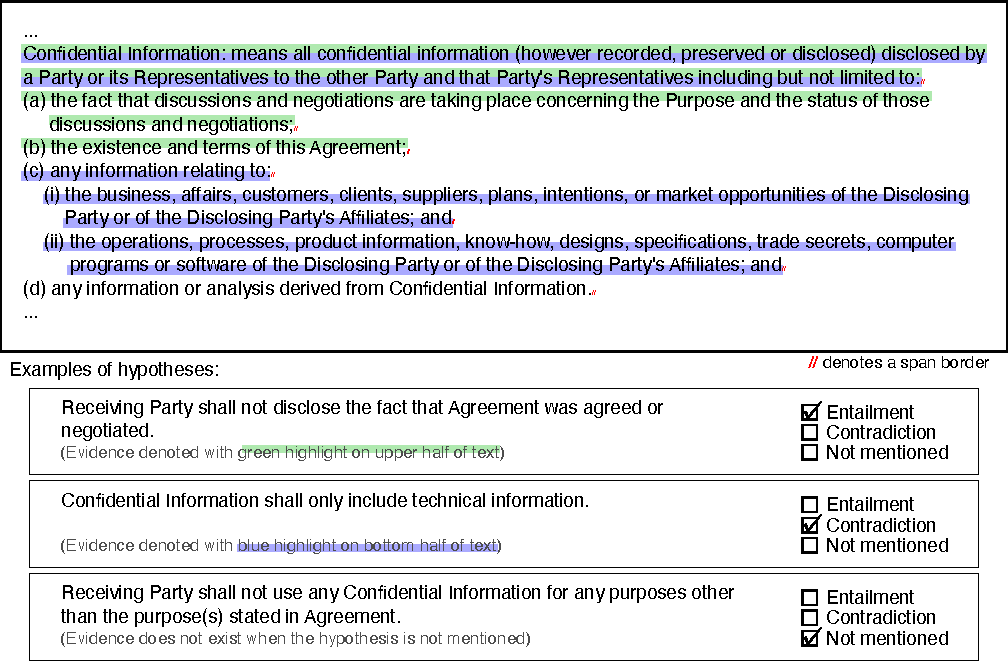
\includegraphics[width=\linewidth]{fig/task_overview}
    \caption{An overview of document-level NLI for contracts. Given a contract, a system must classify whether each hypothesis is \emph{entailed by}, \emph{contradicting to} or \emph{not mentioned by} the contract and identify \emph{evidence} for the decision as spans in the contract.}\label{fig:task_overview}
\end{figure}

Reviewing a contract is a time-consuming procedure.
A study \cite{exigent_group_limited_how_2019} revealed that ``60-80\% of all business-to-business transactions are governed by some form of written agreement, with a typical Fortune 1000 company maintaining 20,000 to 40,000 active contracts at any given time''.
Contract review is carried out manually by professionals, costing companies a huge amount of money each year.
Even worse, smaller companies or individuals may opt for signing contracts without access to such professional services.

To address this need, there is a growing interest in \emph{contract review automation}.
Recently, \citet{leivaditi_benchmark_2020} and \citet{hendrycks_cuad_2021} introduced datasets for extracting certain terms in contracts, which can help a user comprehend a contract by providing a consistent legend for what sort of terms are discussed in the contract.
However, these works only aim to find what sort of terms are present, not what each of such terms exactly states.
For example, \cite{hendrycks_cuad_2021} involves extracting a span in a contract that discusses about a question ``Is there a restriction on a party’s soliciting or hiring employees ...?''.
Being able to answer such questions can further benefit users by automatically detecting terms that are against the user's policy without having have to read each of the extracted terms.

In this paper, we argue that contract review is also a compelling real-world use case for natural language inference (NLI).
However, rather than evaluating a hypothesis versus a short passage, evaluation is against a whole document.
Concretely, given a contract and a set of hypotheses (such as ``Some obligations of Agreement may survive termination.''), we would like to classify whether each hypothesis is \emph{entailed by}, \emph{contradicting to} or \emph{not mentioned by} (neutral to) the contract as well as identifying \emph{evidence} for the decision as spans in the contract (\cref{fig:task_overview}).
Therefore, the problem involves similar evidence identification problems as open domain question answering, a problem less studied in the NLI context, and practical usefulness also involves identifying the evidence spans justifying an NLI judgment.

% Why is it important to linguistic community?
Our work presents a novel, real-world application of NLI.
We further argue that contracts --- which occupy a substantial amount of the text we produce today --- exhibit interesting linguistic characteristics that are worth exploring.
Our contributions are as follows:
\begin{enumerate}
    \item We annotated and release\footnote{\url{https://stanfordnlp.github.io/contract-nli/}} a dataset consisting of 607 contracts. This is the first dataset to utilize NLI for contracts and is also the largest corpus of annotated contracts.
    \item We introduce a strong baseline for our task, Span NLI BERT, which \begin{enumerate*}
        \item makes the problem of evidence identification easier by modeling the problem as multi-label classification over spans instead of trying to predict the start and end tokens, and
        \item introduces more sophisticated context segmentation to deal with long documents
    \end{enumerate*}. We show that Span NLI BERT significantly outperforms the existing models.
    \item We investigate interesting linguistic characteristics in contracts that make this task challenging even for Span NLI BERT.
\end{enumerate}
